\chapter{BIOMOLECULAR SIMULATION: SAMPLING AND FREE ENERGY}

All of the simulation models discussed in Chapter \ref{ch1} use an electrostatic
equation dealing with charges interacting in a vacuum. However, biological
chemistry occurs almost exclusively in an aqueous environment, necessitating the
development of models capable of simulating an aqueous environment for these
systems. In this chapter, we will describe the various methods by which solvent
effects are introduced into simulation, followed by the ensemble sampling
techniques that will be used for the principle studies in this dissertation.

\section{Simulations in the Condensed Phase}

The techniques by which solvation effects can be incorporated into various
computational models can be separated into two groups. The most obvious way is
to include the solvent atoms and molecules directly into the simulation
alongside the system of interest---referred to collectively as \emph{explicit
solvent} methods. While explicit solvent models are the most accurate approach
in principle, they drastically increase the size of the
simulation---simultaneously increasing the cost of the simulation and amount of
sampling required to obtain converged results.

An alternative way to include solvent effects is by modifying the electrostatic
interactions in a system to account for the natural screening that a particular
solvent provides. These approaches are called \emph{implicit solvent} methods
because solvent effects are included in an average way without including the
actual solvent atoms or molecules in the simulation. Simulations employing
implicit solvent models result in smaller simulations in which comformational
sampling converges more rapidly because the solvent degrees of freedom are
already included in a mean field way. However, individual solvent molecules
often play a critical role in the structure and function of biological molecules
and behave very differently than bulk solvent molecules---an effect implicit
solvent models are ill-equipped to handle.

The following sections describe the various implicit and explicit solvent models
commonly used in biomolecular simulations.

\subsection{Implicit Solvent}

One of the most important qualities of a solvent---especially an aqueous
solvent---is its ability to polarize in response to an electric field, thereby
reducing the magnitude of electrostatic interactions across a given distance.
While the na\"ive approach of simply applying the solvent dielectric everywhere
is attractive in its simplicity, solvent-excluded regions should obviously not
be subject to the screening effects of the solvent. For large biomolecules, the
solvent-excluded regions can be very large, so it becomes very important to deal
with these regions effectively.

\subsubsection{Distance-dependent Dielectric}

Among the earliest approaches to account for the different dielectric
environments of a bimolecule interior and bulk solvent introduced a dielectric
constant that changed as a function of the distance between two charged
particles. As the separation between two particles increased, so too did the
likelihood that they were separated by solvent, and so were subject to
dielectric screening effects.

This approach is attractive in its simplicity---it adds little to the
computational cost of the model while retaining the simple,
pairwise-decomposable nature of the electrostatic potential term. A common
equation modeling the dielectric constant is given below in Eq.
\ref{eq2:DistanceDielectric}. \cite{Leach_Book_MolModel_2001}

\begin{equation}
   \varepsilon _ {eff} (r) = \frac {\varepsilon_{bulk} - 1} 2 \left [ (rS) ^2 +
   2rS + 2 \right ] \exp(-rS)
   \label{eq2:DistanceDielectric}
\end{equation}
where $r$ is the distance between the two particles, $\varepsilon_{bulk}$ is the
dielectric constant of the bulk, $\varepsilon_{eff}$ is the effective
dielectric constant at a given particle separation, and $S$ is a free parameter.
Fig. \ref{fig2:DistanceDielectric} plots the resulting curve for
$\varepsilon_{eff}$ from Eq. \ref{eq2:DistanceDielectric} for different values
of the free parameter.

\begin{figure}
   \includegraphics[width=6.5in]{DistanceDielectric.ps}
   \caption{Distance-dependent dielectric for different values of the free
            parameter $S$ in Eq. \ref{eq2:DistanceDielectric}.}
   \label{fig2:DistanceDielectric}
\end{figure}

This effective dielectric constant is then incorporated as $\epsilon$ in Eq.
\ref{eq1:AmberFF2}, and influences the calculated forces due to its dependence
on $r_{i,j}$. One of the biggest weaknesses of distance-dependent
dielectrics is that it treats every atom in the biomolecule as though they are
in the same environment, and the shapes of biomolecules---and their
solvent-excluded volumes---are often highly irregular. That is, two atoms buried
inside the solvent-excluded volume separated by $d$ {\AA} are treated exactly
the same way as two different atoms $d$ {\AA} apart whose interstitial region is
solvent-accessible. Furthermore, because the shapes of biomolecules can vary
greatly from system to system, the `optimal' value for $S$ in Eq.
\ref{eq2:DistanceDielectric} is highly system-dependent. Finally, while the true
dielectric regions are either the value of the bulk solvent or the molecule
interior, a distance-dependent dielectric has a large region corresponding to
unphysical, intermediate values of the dielectric.

For these reasons, the distance-dependent dielectric model is rarely used in
modern simulations, having given way to the more accurate methods like the
Poisson-Boltzmann equation and Generalized Born equation.

\subsubsection{Poisson-Boltzmann}

At the heart of all modern implicit solvent models lies the Poisson equation
\begin{equation*}
   \bigtriangledown \epsilon(\vec{r}) \, \bigtriangledown \phi ( \vec{r} ) =
            -\frac {4 \pi \rho(\vec{r})} {\epsilon ( \vec{r} )}
\end{equation*}
where $\phi$ is the electrostatic potential at a given point in space, $\rho$ is
the charge distribution at a given point in space, and $\epsilon$ is the
dielectric constant at a given point in space. The dielectric constant is often
divided into two regions---a region of low dielectric in the solvent-excluded
volume and that of the bulk solvent `outside' the system of interest.
\cite{Cramer_Book_EssentialsCompChem_2004}

The Poisson equation is only valid, however, at zero ionic strength. When mobile
ions are present---as is the case \emph{in vivo} with all biomolecules---the
Poisson equation must be augmented with an appropriate distribution of
counterions. The probability of finding an ion in a particular region of space
is related to its Boltzmann factor $\exp (-\beta q \phi(\vec{r}))$, where $q
\phi(\vec{r})$ is the energy of a point charge in a given electrostatic
potential. Because ions come in pairs with both positive and negative charges,
the Boltzmann probability of finding both types of ions must be included. The
equation for calculating the electrostatic potential in a biomolecular system
with a given solution ionic strength, termed the \emph{Poisson-Boltzmann} (PB)
equation, is shown in Eq. \ref{eq2:PoissonBoltzmann}.
\cite{Cramer_Book_EssentialsCompChem_2004}

\begin{align}
   \bigtriangledown \epsilon(\vec{r}) \cdot \bigtriangeldown \phi(\vec{r}) -
      \epsilon(\vec{r}) \lambda(\vec{r}) \kappa^2 \frac{k_B T} {2 q} \exp \left
      ( -\beta q \phi(\vec{r}) \right ) -  \epsilon(\vec{r}) \lambda(\vec{r})
      \kappa^2 \frac{k_B T} {2 q}  \exp \left ( \beta q \phi(\vec{r}) \right )
      \right ] & = -4 \pi \rho (\vec{r}) \nonumber \\
   \bigtriangledown \epsilon(\vec{r}) \cdot \bigtriangledown \phi(\vec{r}) -
      \epsilon(\vec{r}) \lambda(\vec{r}) \kappa^2 \frac{k_B T} q \sinh \left (
      \frac {q \phi(\vec{r})} {k_B T} \right ) & = -4 \pi \rho (\vec{r})
   \label{eq2:PoissonBoltzmann}
\end{align}
where $q$ is the charge of the ions (both positive and negative ions are
present), $\lambda(r)$ is a simple switching function that is 0 in
solvent-excluded regions and 1 in solvent-accessible regions, and $\kappa^2$ is
related to the ionic strength as
\begin{equation*}
   \kappa ^ 2 = \frac {8 \pi q ^ 2 I} {\epsilon k_B T}
\end{equation*}

Eq. \ref{eq2:PoissonBoltzmann} is a non-linear, second-order differential
equation in the electrostatic potential that must be solved iteratively until
the desired level of self-consistency in the electrostatic potential is
achieved. The $\sinh$ term in Eq. \ref{eq2:PoissonBoltzmann} may be expanded
using its Taylor series expansion. If the ionic strength is low and the solute
is not highly charged (so $\phi(\vec{r})$ is relatively small), the Taylor
series expansion for $\sinh$ can be truncated after the first term to yield the
much simpler Eq. \ref{eq2:LinearPB} with little loss of accuracy. Eq.
\ref{eq2:LinearPB} is called the \emph{linearized} Poisson-Boltzmann equation
because the Taylor series expansion for $\sinh(x)$ is truncated after its linear
term, $x$.

\begin{equation}
   \bigtriangledown \epsilon (\vec{r}) \bigtriangledown \phi(\vec{r}) -
         \epsilon(\vec{r}) \lambda(\vec{r}) \kappa ^ 2 \phi(\vec{r}) = -4 \pi
         \rho(\vec{r})
   \label{eq2:LinearPB}
\end{equation}

The Poisson Equation can be solved for only the simplest systems, like solvating
a point-charge or a conducting sphere with a uniform charge distribution on its
surface. Eq. \ref{eq2:PoissonBoltzmann} or \ref{eq2:LinearPB} must be solved
numerically for complex biomolecules with irregular shapes. A common approach is
to set up a three-dimensional grid surrounding the solute and calculate the
charge distribution on the grid from the partial charges of each solute atom.
The dielectric boundary can be calculated from the solvent accessible surface
\cite{Sitkoff_JPhysChem_1994_v98_p1978}, so each grid point has an associated
charge and dielectric value. The differential equations can then be solved via
finite differences within the defined grid. \cite{Klapper_Proteins_1986_v1_p47}

After the electrostatic potential is calculated via Eq.
\ref{eq2:PoissonBoltzmann}, the free energy is calculated by integrating the
product of the charge distribution and the calculated electrostatic potential
according to
\begin{equation*}
   G = \frac 1 2 \int \rho(\vec{r}) \phi(\vec{r}) d\vec{r}
\end{equation*}
where the $1/2$ factor corrects for double-counting the interactions.  The free
energy of solvation due to solvent polarization is calculated from the
difference in the electrostatic potentials in vacuum and solvent ($\phi_{solv} -
\phi_{vac}$)---a quantity referred to as the \emph{reaction field}.
\cite{Leach_Book_MolModel_2001}

Models employing implicit solvent via the PB equation have proven
effective in many cases. \cite{Klapper_Proteins_1986_v1_p47,
Gilson_JComputChem_1988_v9_p327, Baker_ProcNatlAcadSci_2001_v98_p10037,
Nielsen_Proteins_2001_v43_p403} However, due to requirements of a fairly dense
grid and the iterative, self-consistent solution of the PB equation, the
computational cost of this model is too high for many applications. Furthermore,
the dielectric function is discontinuous at the boundaries of the
solvent-excluded and solvent-accessible regions, making stable gradients (and
therefore forces) difficult to calculate. Therefore, we now consider a common
approximation to the PB equation called the \emph{Generalized Born} model that
seeks to provide an efficient, analytical alternative to solving the PB
equation.

\subsubsection{Generalized Born}

\subsection{Explicit Solvent}

\subsubsection{Periodic Boundary Conditions}

\subsubsection{Cutoff Methods}

\subsubsection{Ewald Summation}

\paragraph{Particle-Mesh Ewald}

\subsubsection{Other Approaches}


